\documentclass[aspectratio=169]{beamer}
\usepackage[T1]{fontenc} \usepackage{lmodern} \usepackage[utf8]{inputenc}
\usepackage[english]{babel} \usepackage{booktabs}
\usepackage{graphicx,subcaption} \usepackage{amssymb,amsmath}
\graphicspath{{figures/}}
\usepackage[citestyle=authoryear,bibstyle=authoryear,backend=biber,url=false,doi=false,isbn=false]{biblatex} \bibliography{refs}
\usepackage{hyperref}

% Make Adobe Reader use the RGB rendering model for pages with transparency.
\pdfpageattr{/Group << /S /Transparency /I true /CS /DeviceRGB>>}

\mode<presentation>{
	\usetheme{Malmoe}
	\usecolortheme{beaver}
	\setbeamertemplate{footline}[page number]
	\setbeamertemplate{navigation symbols}{}
}

%------------------------------------------------

\DeclareMathOperator*{\diag}{diag}
\DeclareMathOperator*{\argmin}{arg\,min}
\DeclareMathOperator*{\spn}{span}
\newcommand{\G}{\mathcal{G}}
\newcommand{\V}{\mathcal{V}}
\newcommand{\E}{\mathcal{E}}
\newcommand{\bO}{\mathcal{O}}
\newcommand{\R}{\mathbb{R}}

\newcommand{\good}[1]{{\color[rgb]{0.2,0.6,0.2}#1}}
\newcommand{\bad}[1]{{\color{red}#1}}
\newcommand{\txt}[1]{\hspace{.5cm} \text{#1} \hspace{.5cm}}
\newcommand{\define}[1]{\item{\usebeamercolor[fg]{enumerate item}#1}:}
\newcommand{\HRule}{{\usebeamercolor[bg]{subsection in head/foot} \rule{\linewidth}{0.5mm}}}

%------------------------------------------------

\begin{document}

\begin{frame}[plain]
	%\titlepage
	\begin{center}

		\begin{minipage}{0.7\linewidth}
			\textsc{\large A Network Tour of Data Science}
		\end{minipage}
		\hfill
		\begin{minipage}{0.25\linewidth}
			
\includegraphics[width=\linewidth]{logo_epfl}
		\end{minipage}
		\vspace{0.5cm}

		\HRule
		\vspace{0.55cm}
		{
			\usebeamercolor[fg]{frametitle}
			\textsc{\Large Projects}\\
			\vspace{0.3cm}
		}
		\HRule
		\vspace{0.8cm}

		\hspace{0.5cm}
		\begin{minipage}{0.4\linewidth}
			\footnotesize
			\textbf{Teachers} \\
			Pierre \textsc{Vandergheynst} \\
			Pascal \textsc{Frossard} \\
		\end{minipage}
		\begin{minipage}{0.4\linewidth}
			\footnotesize
			\textbf{Assistants} \\
			Michaël \textsc{Defferrard} \\
			Effrosyni \textsc{Simou} \\
			Hermina \textsc{Petric Maretić} \\
			Rodrigo \textsc{Pena} \\
			Eda \textsc{Bayram} \\
			Benjamin \textsc{Ricaud} \\
		\end{minipage}

		\vspace{0.4cm}
		{\footnotesize EPFL LTS2 \& LTS4 laboratories
		\hfill December 5, 2018}

	\end{center}
\end{frame}

%------------------------------------------------

\begin{frame}
	\frametitle{Goal}
	The milestones gave you
	\vspace{0.5em}
	\begin{itemize}
		\item an understanding of your data,
		\item practical experience with some tools.
	\end{itemize}
	\vfill
	Use that knowledge to
	\vspace{1em}
	\begin{center}
		\huge
		tell us a data story.
	\end{center}
\end{frame}

%------------------------------------------------

\begin{frame}
	\frametitle{Process}
	\begin{enumerate}
		\item Define a problem.
		\item Use your dataset to solve it.
		\item Use the tools seen during the course.
		\item Present your conclusions.
	\end{enumerate}
	\vfill
	Beware:
	\begin{itemize}
		\item Set a goal that is attainable given your understanding of the data and tools.
		\item It's not a presentation about what you did during the milestones!
		\item Projects should use tools and ideas from the lectures. They should include graph and network data aspects, and more generally fall under the scope of the class.
		\item Building a good graph is as important as analyzing it. Your graph should be built towards the goal of solving your problem.\footnote{We didn't care much for the milestones as there was no real problem to solve.} That includes sub-sampling.
	\end{itemize}
\end{frame}

%------------------------------------------------

\begin{frame}
	\frametitle{Two directions}
	\begin{itemize}
		\item Use the data to answer a research question you are curious about.
		\vfill
		\item Use the data to build a ``product'', e.g., predict some variables given others.
	\end{itemize}
\end{frame}

%------------------------------------------------

\begin{frame}
	\frametitle{Examples}
	\begin{description}
		\item[IMDb] How do actors choose a film to play with? Do they form communities? What are the characteristics of those communities?
		\item[FMA] Can an online music platform recommend annotations (such as tags or genres) to artists regarding their newly uploaded songs?
		\item[Senators] Are senators truly divided in republicans and democrats? Can I predict the votes of a senator knowing the votes of ``similar'' senators?
	\end{description}
	\vfill
	Good examples from last year:\footnote{available at \url{https://github.com/mdeff/ntds_2017}}
	\vfill
	\begin{minipage}{0.60\linewidth}
		\begin{itemize}
			\item A Network Tour of StackOverflow
			\item GSP on the Digital Reconstruction of the Brain
			\item Graph-based Recommendation for lastFM
		\end{itemize}
	\end{minipage}
	\hfill
	\begin{minipage}{0.39\linewidth}
		\begin{itemize}
			\item Graph-based Nutrition Guide
			\item Buda + Pest = Budapest
			\item GraphLang
		\end{itemize}
	\end{minipage}
\end{frame}

%------------------------------------------------

\begin{frame}
	\frametitle{Deliverables}
	\begin{description}
		\item [report] Describe your motivations, explain what you did and why (e.g., how you built the graph and why), and state your conclusions. The report contains an exploration part (e.g., some important or interesting facts about your data and graph), and an exploitation part (how you used the data to solve your problem). The report is a 5 pages PDF.
		\vfill
		\item [code] All the code you developed for the project must be stored in a GitHub repository. It should contain a useful readme and a license. Code should be organized and clean.
		\vfill
		\item [presentation] Impress us! Presentations are 12 minutes long, followed by 3 minutes of questions. Each group member must talk.
	\end{description}
\end{frame}

%------------------------------------------------

\begin{frame}
	\frametitle{Deadlines}
	\begin{description}
		\item[Jan 18] upload the project report on Moodle
		\vfill
		\item[Jan 18] send a link to your GitHub
		\vfill
		\item[Jan 22-23] give an oral presentation
		\vfill
		\item[Jan 25] upload the presentation slides on Moodle
	\end{description}
\end{frame}

%------------------------------------------------

\begin{frame}
	\begin{center}
		\Huge Have fun!
		\hspace{2em}
		\Huge Questions?
	\end{center}
	\begin{figure}
		\centering
		\begin{subfigure}[b]{0.24\linewidth}
			
\includegraphics[width=\linewidth]{project2017_brain}
		\end{subfigure}
		\hfill
		\begin{subfigure}[b]{0.24\linewidth}
			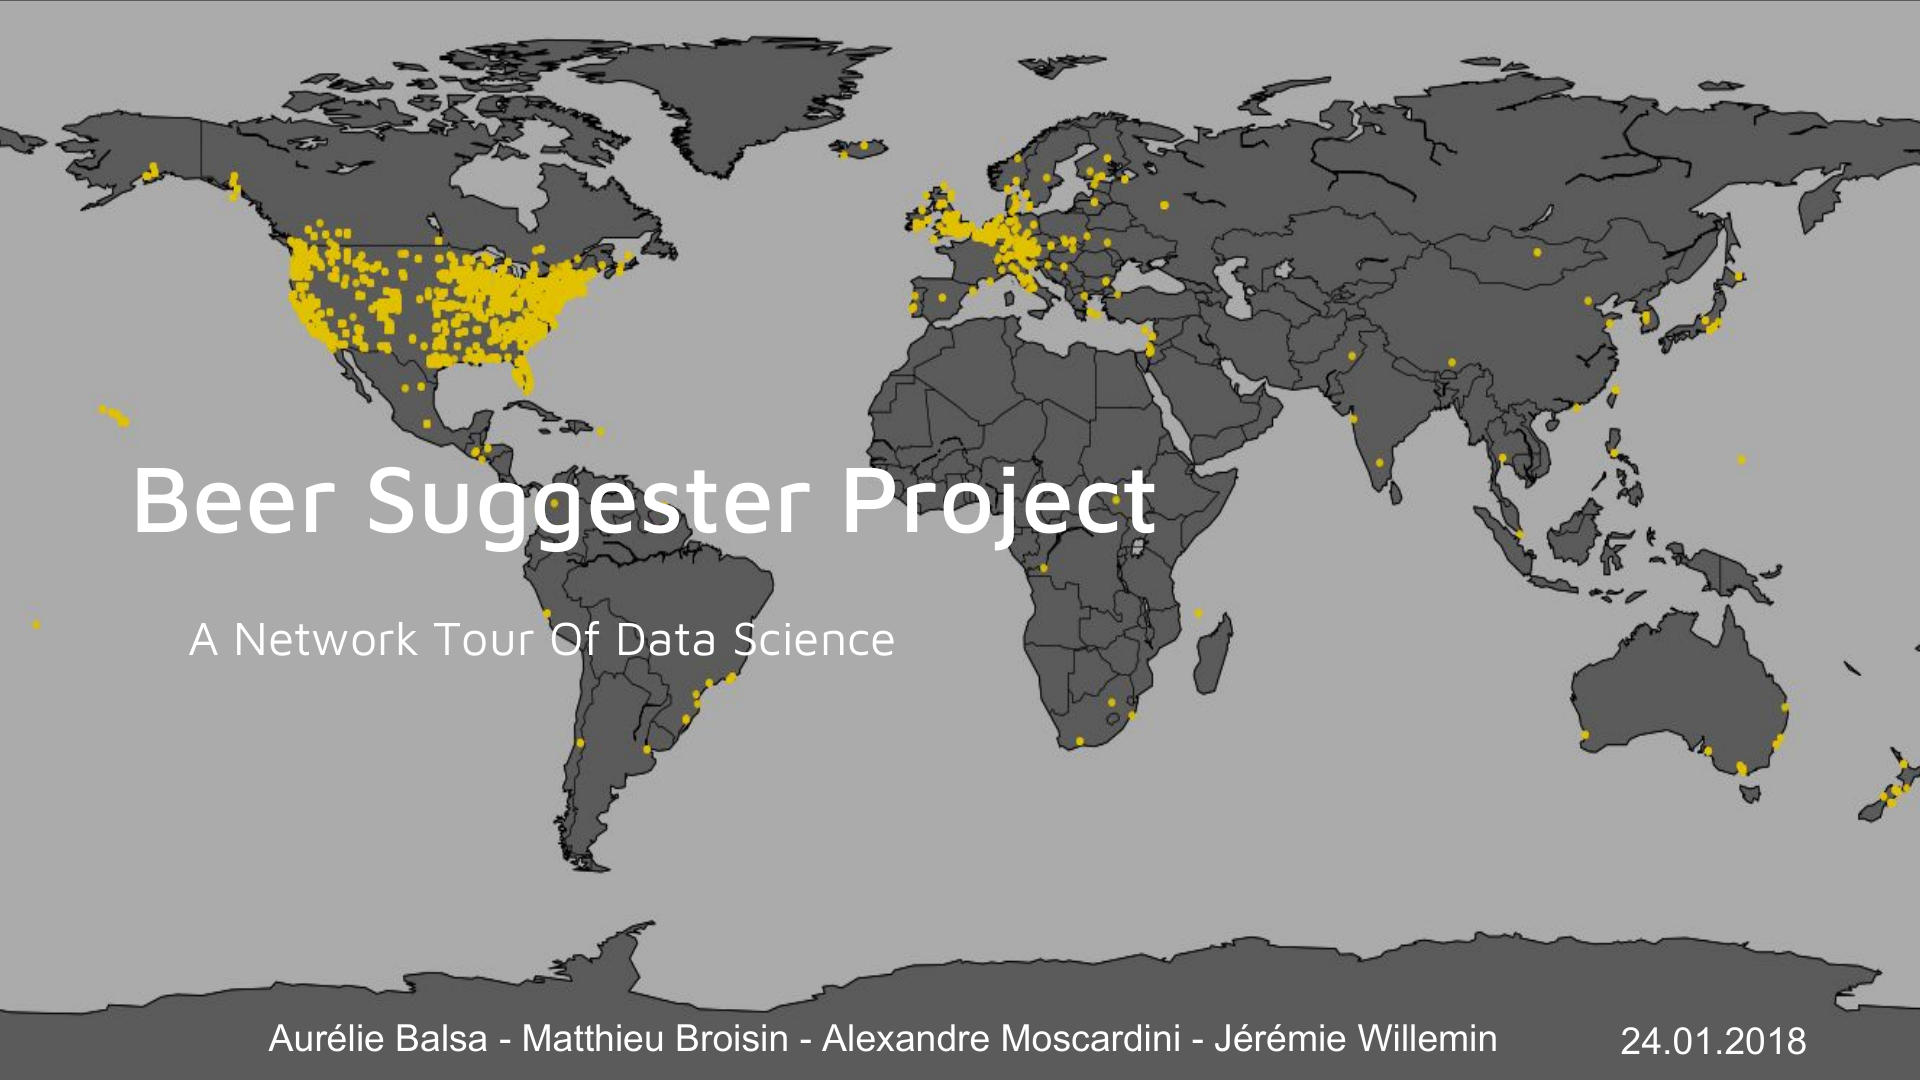
\includegraphics[width=\linewidth]{project2017_beer}
		\end{subfigure}
		\hfill
		\begin{subfigure}[b]{0.24\linewidth}
			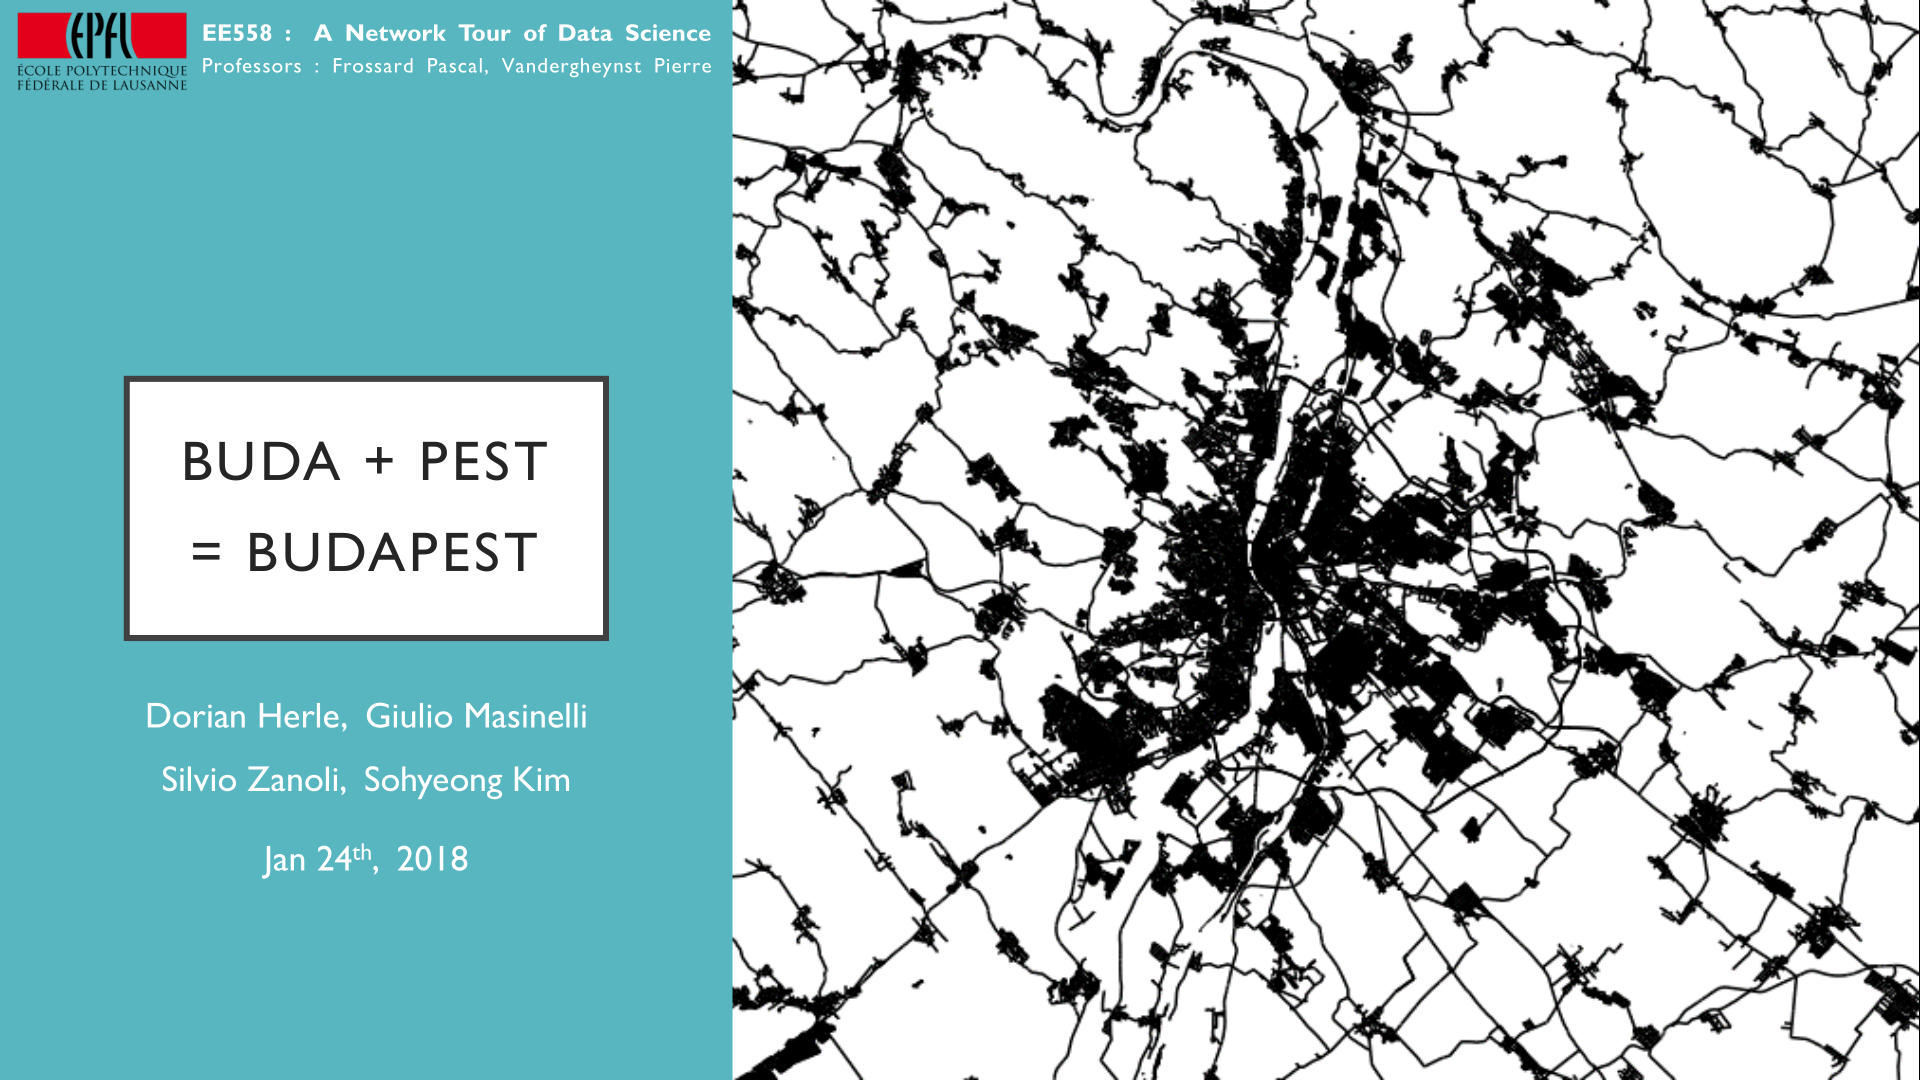
\includegraphics[width=\linewidth]{project2017_roads}
		\end{subfigure}
		\hfill
		\begin{subfigure}[b]{0.24\linewidth}
			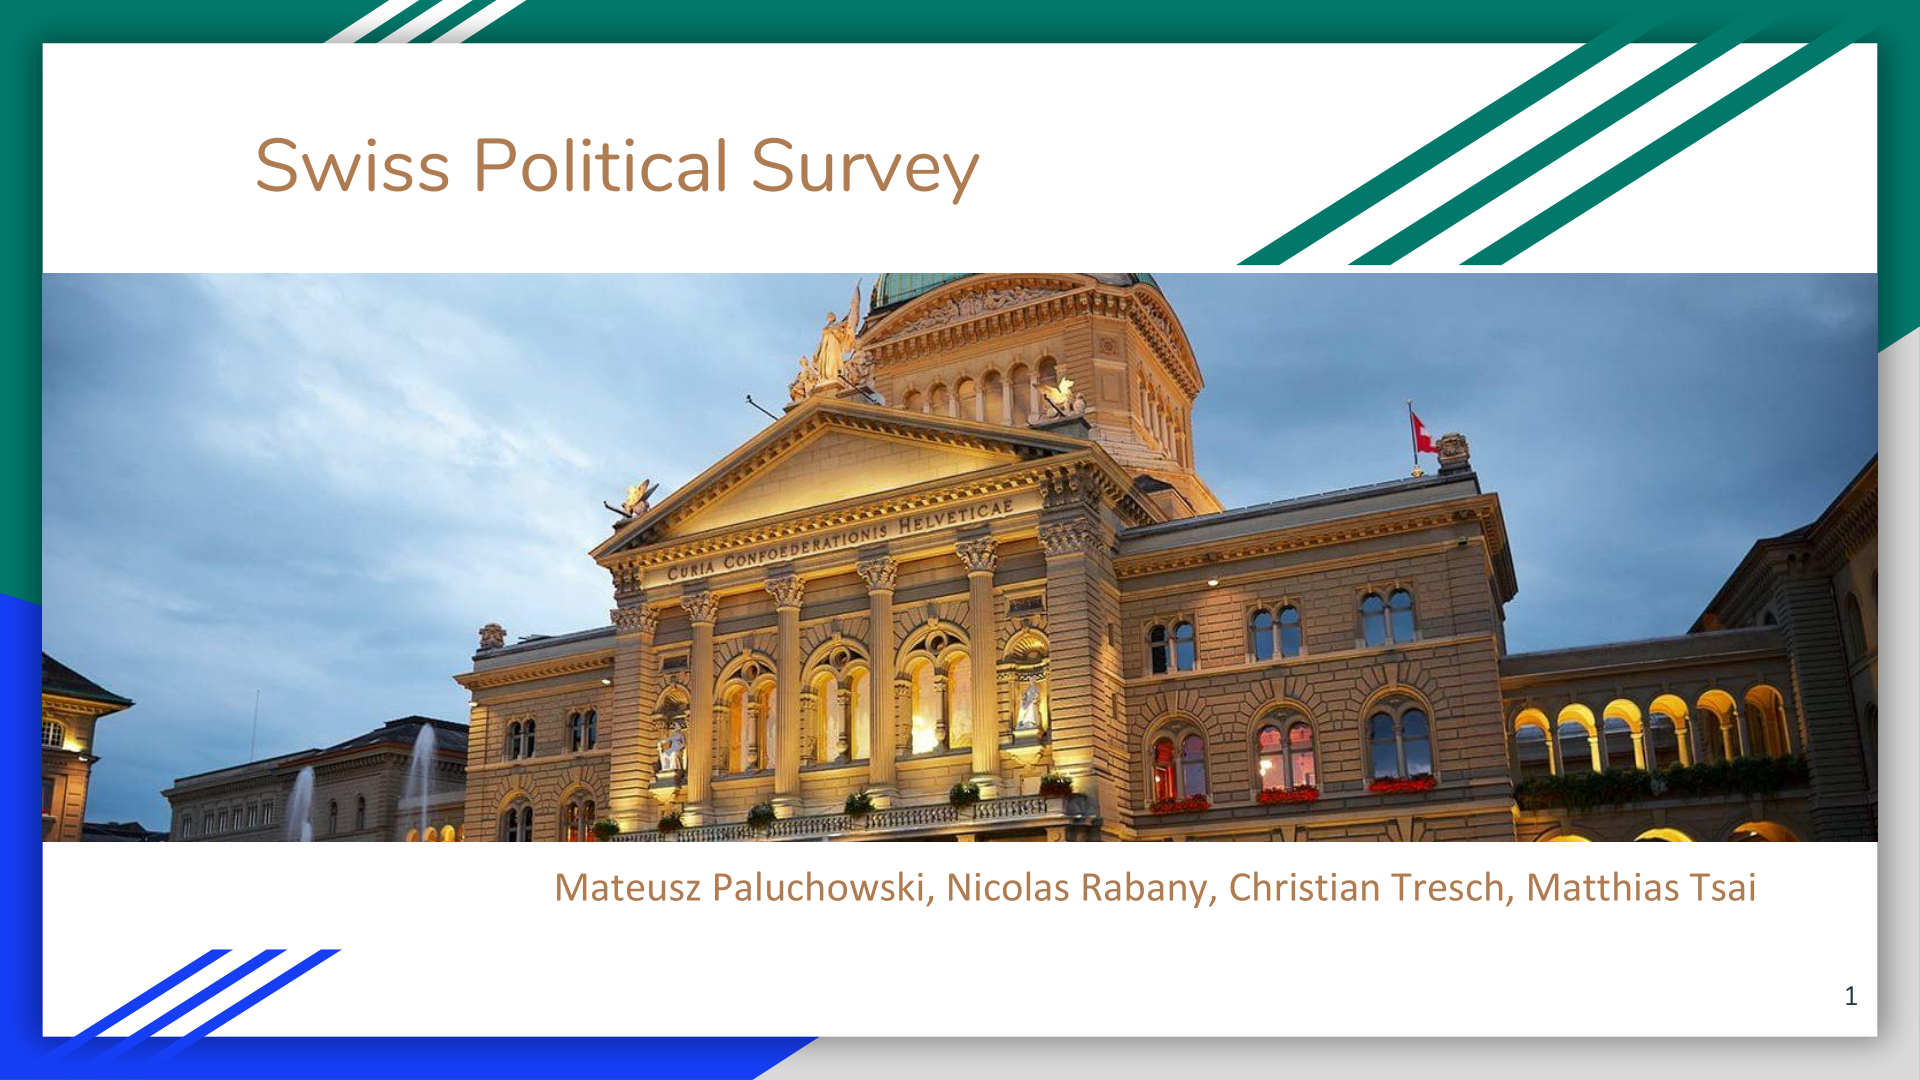
\includegraphics[width=\linewidth]{project2017_politics}
		\end{subfigure}
		\\
		\vspace{2em}
		\begin{subfigure}[b]{0.24\linewidth}
			
\includegraphics[width=\linewidth]{project2017_stackoverflow}
		\end{subfigure}
		\hfill
		\begin{subfigure}[b]{0.24\linewidth}
			
\includegraphics[width=\linewidth]{project2017_springs}
		\end{subfigure}
		\hfill
		\begin{subfigure}[b]{0.24\linewidth}
			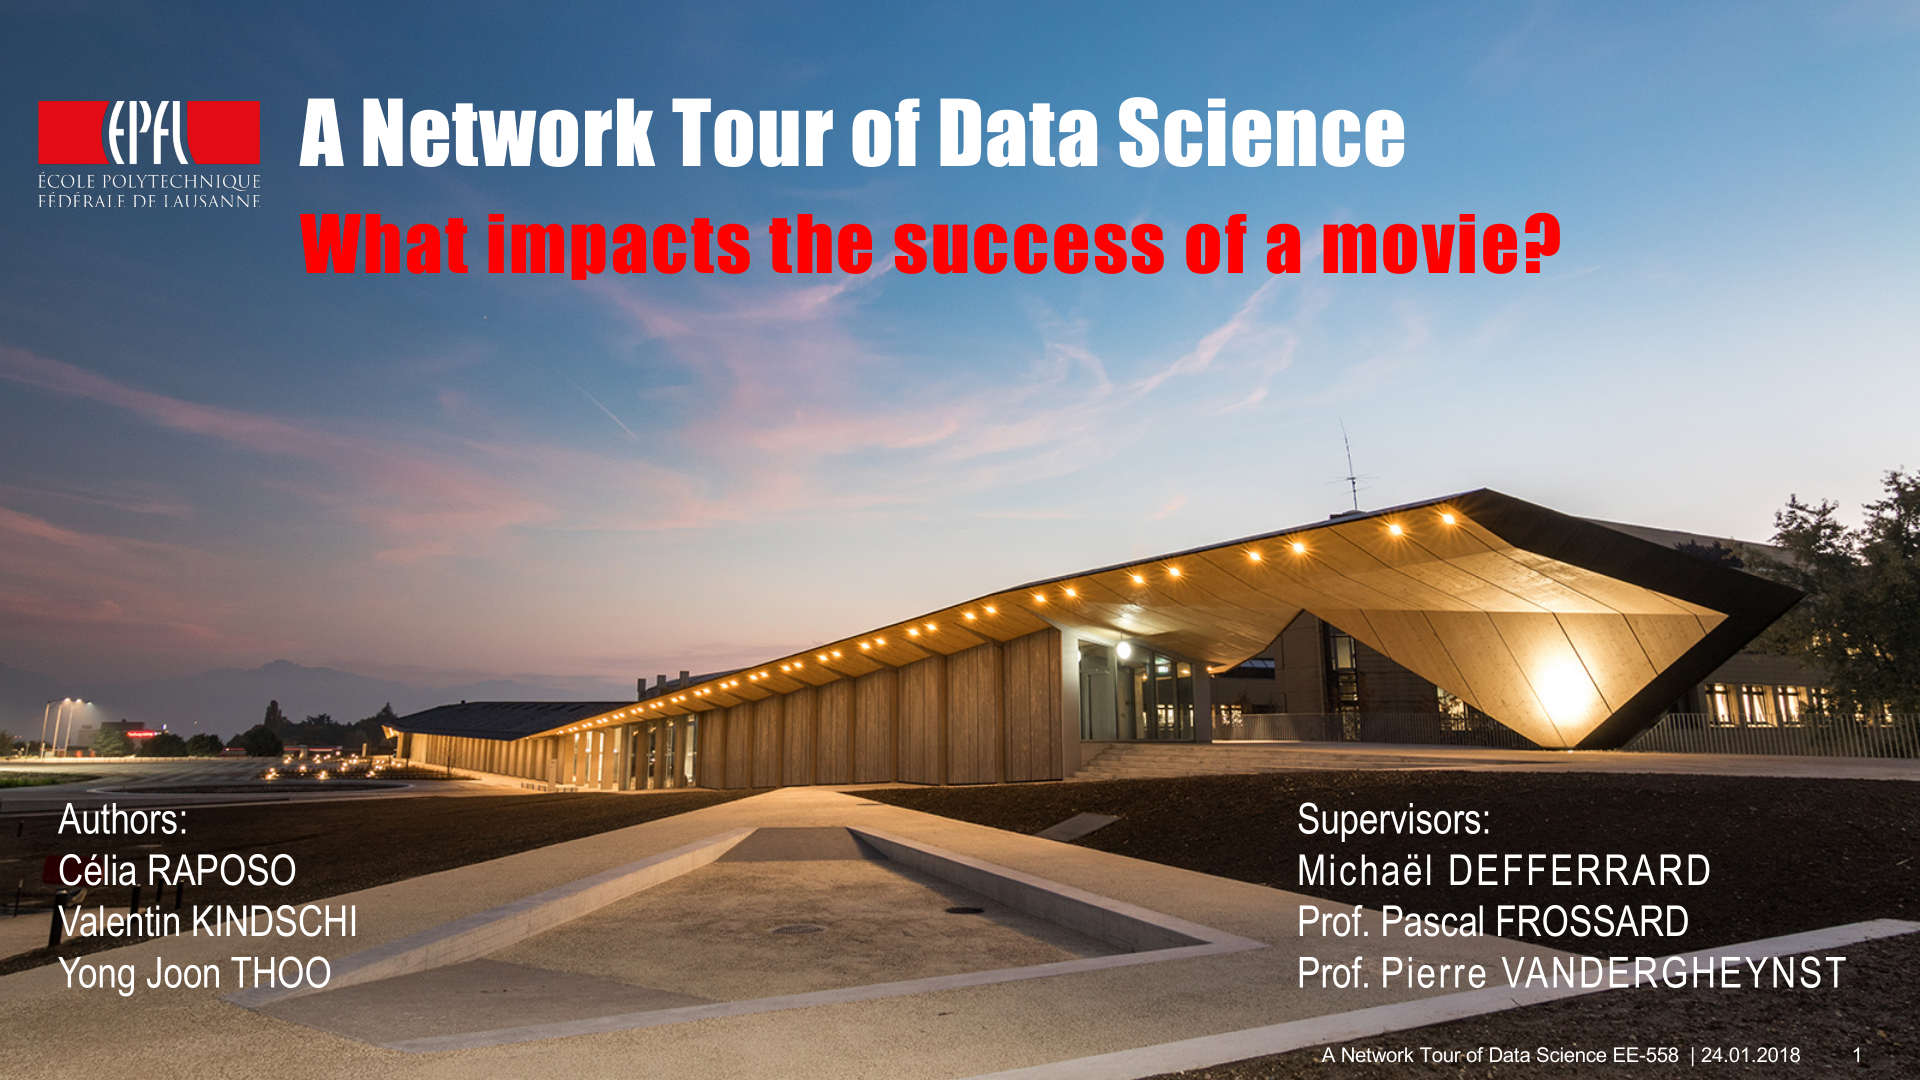
\includegraphics[width=\linewidth]{project2017_movies}
		\end{subfigure}
		\hfill
		\begin{subfigure}[b]{0.24\linewidth}
			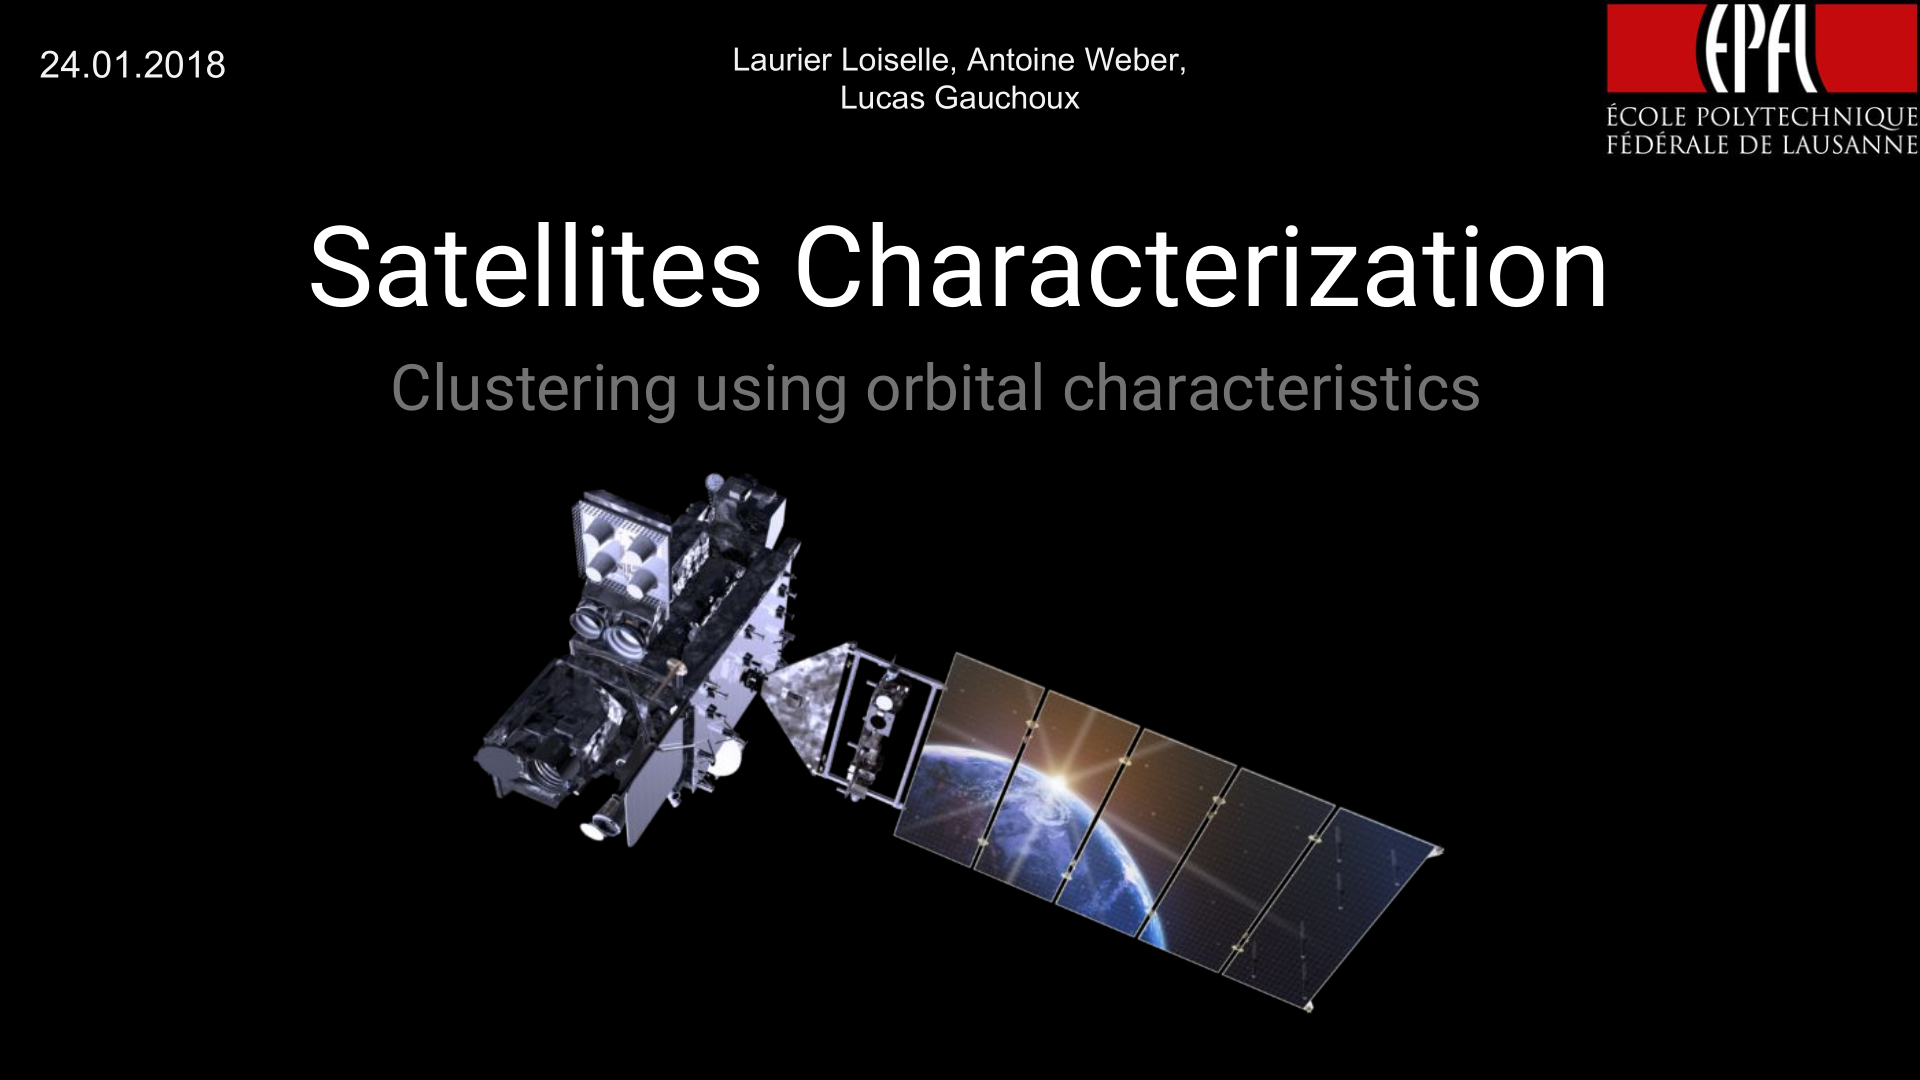
\includegraphics[width=\linewidth]{project2017_satellites}
		\end{subfigure}
	\end{figure}
\end{frame}

%------------------------------------------------

\end{document}
